\documentclass{article}
\usepackage[utf8]{inputenc}
\usepackage[margin=1in]{geometry}
\usepackage{mathtools,setspace,indentfirst,graphicx,float,hyperref,courier,color,times}
\usepackage{fancyhdr} % for header
\usepackage{listings}
\usepackage{csquotes}
\usepackage[american]{babel}
\usepackage[backend=biber,citestyle=numeric,bibstyle=apa]{biblatex}
%\bibliographystyle{apacite}
%\addbibresource{sources.bib}
\DeclareLanguageMapping{american}{american-apa}
\bibliography{sources}

\doublespacing{}

\fancyhf{}
\pagestyle{fancy}

\lhead{N Batista, M Inciong, F Truncale}
\chead{\thepage}
\rhead{Fall 2017}
\renewcommand{\headrulewidth}{0pt} % remove the horizontal line along the header
% figure numbering you can actually follow
% only downside is you need to reset the counter every subsection
\renewcommand{\thefigure}{\arabic{section}.\arabic{subsection}.\arabic{figure}} 

\lstset{%
  basicstyle=\ttfamily,
  captionpos=b,
  frame=tb,
  tabsize=2,
  showstringspaces=false,
  commentstyle=\color[RGB]{24,135,64},
  keywordstyle=\color{blue},
  stringstyle=\color{red}
}

\begin{document}

\thispagestyle{empty}

\begin{titlepage}
  \vspace*{\fill} % i copied this off stackexchange so no i don't know what that asterisk does.
  \begin{center}
    {\Huge Final Report --- Optimization of Subgraph Isomorphism Algorithm}\\[0.4cm]
    {\huge by Nelson Batista, Max Inciong, Francesca Truncale}\\[0.5cm]
    {\huge Senior Project II}\\[0.4cm]
    {\huge Professor Jianting Zhang}\\[0.4cm]
    {\LARGE Fall 2017}
  \end{center}
  \vspace*{\fill}
\end{titlepage}

\pagenumbering{roman}
%table of contents
\tableofcontents

\newpage

\pagenumbering{arabic}
\setcounter{page}{1}

%\addcontentsline{toc}{section}{Introduction}
\section{Introduction}

The goal of this project is to understand and optimize an algorithm for solving the NP-complete problem of subgraph isomorphism.

  \subsection{Background}

  An \textit{isomorphism} between two graphs is a mapping from the vertices of one graph, say $G$, to another graph, say $H$, such that any two vertices which are adjacent in $G$ are mapped to vertices which are adjacent in $H$. The subgraph isomorphism problem, in turn, is the problem of determining whether an isomorphism exists between a graph $G$ and any of the subgraphs of a larger search graph, $H$. The issue that makes the subgraph isomorphism problem so difficult to solve for a particular pair of graphs is cycling through the main graph and expanding each node within the graph and checking if each of the generated subgraphs formed from each node is isomorphic to the control graph.

  Fortunately, many attempts exist to solve the subgraph isomorphism problem. Among the earliest of these is the famous \textit{Ullmann Algorithm}, proposed by Julian R. Ullmann in his 1976 paper, \textit{An Algorithm for Subgraph Isomorphism}. He first describes a basic, naive approach to finding a mapping from the vertices of a graph to a subgraph of a larger graph. He goes on to define a ``refine'' procedure to dramatically reduce the number of possible mappings that must be checked.\cite{ullmann} These will be covered in greater detail in the next section.

  The goal of our project was to take this algorithm and improve its performance. Subgraph isomorphism is an expensive problem to solve, and finding multiple possible isomorphisms from one graph to subgraphs of another is even more expensive, so even slight improvements in the algorithm's performance is likely to lead to large performance improvements in any large-scale program which needs to use it often.

  \subsection{Motivation}

  Our reasoning for choosing this topic for our project is an apparent lack of especially efficient algorithms for solving the subgraph isomorphism problem. Solutions to the subgraph isomorphism problem are often used to detect similarities in chemical compounds,\cite{ullmann} which may shed light on some of their properties. If this process needs to be done, for example, on a very large database of chemical compounds, or less frequently for several very large compounds, the process may take a very long time to complete. It would be very beneficial to improve the performance of this algorithm, even if only slightly, so that these sorts of use cases can still be handled in a more reasonable amount of time.

  \subsection{Data Set}

  The primary graph used to test the algorithm and its performance is an undirected graph consisting of ``friends lists'' from the social media website, Facebook. Each node of the graph represents a unique user, and, if two nodes are adjacent, then their corresponding users are friends on Facebook.\cite{fbgraph}

  The graph contains 4,039 nodes and 88,234 edges. The relatively large size of the graph makes it well-suited to use for collection of performance data. As we shall see, the Ullmann algorithm takes a rather long time to complete with a graph of this size, allowing any optimizations and/or parallelizations to be readily apparent.

\section{Ullmann Algorithm}

  \subsection{Naive Approach}

  The paper begins, as many do, with a definition of terms that will be used throughout. We have repeated them here for the sake of clarity later on. We begin by noting that the algorithm models the search for a possible mapping by having all possible mappings as nodes on a tree, on which a depth-first search is performed to find a solution.

  The subgraph isomorphism problem is defined as the problem of finding all isomorphisms between a graph $G_\alpha = (V_\alpha, E_\alpha)$ and subgraphs of another graph $G_\beta = (V_\beta, E_\beta)$, with $(V_\alpha, E_\alpha)$ and $(V_\beta, E_\beta)$ being the set of vertices and edges of $G_\alpha$ and $G_\beta$, respectively. The number of vertices and edges of $G_\alpha$ and $G_\beta$, respectively, are $(p_\alpha, q_\alpha)$ and $(p_\beta, q_\beta)$.

  The \textit{adjacency matrix} for graph $G_\alpha$, $[a_{ij}]$, is defined by:

  \[ a_{ij} = \begin{cases}
                1 & \textrm{ if } i \neq j \textrm{ and } i,j \textrm{ share an edge} \\
                0 & \textrm{ otherwise}
  \end{cases}
  \]

  The adjacency matrix for graph $G_\beta$, $[b_{ij}]$, is defined equivalently.

  Notably, we have the $p_\alpha \times p_\beta$ matrix $M$, which is a binary matrix of assignments (mappings) from $V_\alpha$ to $V_\beta$. That is, if $m_{ij}$ is 1, then vertex $i$ in graph $G_\alpha$ could possibly be mapped to vertex $j$ in $G_\beta$. Otherwise $m_{ij}$ is 0. M has a few interesting properties as a result, which will soon be apparent.

  Finally, we come to $d$, which is simply algorithm's current depth in the search tree. The algorithm starts at $d = 0$, and terminates when $d = p_\alpha$. The matrix $M$ at a particular depth $d$ is denoted as $M_d$, with solutions to the working instance of the subgraph isomorphism problem being the set of assignments from $V_\alpha$ to $V_\beta$, contained within matrices $M_{p_\alpha}$. $M_0$ is generated by the following formula:

  \[ m_{ij} = \begin{cases}
    1 & \textrm{ if degree} (j \in G_\beta) \geq \textrm{ degree} (i \in G_\alpha) \\
                0 & \textrm{ otherwise}
  \end{cases}
  \]

  Each step of the computation consists of setting all but one of the values of one of the rows of $M$ to 0, and then checking whether exactly one 1 exists in each row. If it does, we have found an isomorphism, since each vertex of $G_\alpha$ has been mapped to exactly one vertex of $G_\beta$. If it does not, then we continue onto another row of $M$ and check again. If we have reached the point where we cannot perform the operation on a row of $M$ without violating the condition that each \textit{column} of $M$ contains at most a single 1 (a vertex of $G_\beta$ cannot be mapped from multiple vertices of $G_\alpha$), then we backtrack to a previous version of $M$ and try to change the column that we set to 1 in the current row. After exhausting all columns, we conclude there cannot be an isomorphism, since at least one vertex of $G_\alpha$ cannot be mapped to any vertex of $G_\beta$.\cite{ullmann}

  \subsection{``Refine M'' Procedure}

  In the naive algorithm, the entire tree is searched, including branches which cannot possibly contain a solution at any depth. This is a large number of $M$ matrices to evaluate, so Ullmann introduces a ``refine M'' procedure to reduce the number that must be checked by eliminating nodes of the tree, and thus all of their child nodes, which cannot contain a solution.

  The procedure is actually quite simple. We iterate through each 1 $m_{ij}$ in $M$ and check whether, for each neighbor of the vertex in $G_\alpha$ corresponding to $i$, there exists at least one possible assignment from it to a neighbor of the vertex in $G_\beta$ corresponding to $j$. If this condition does not hold, the 1 is changed to a 0. Since doing so may render other 1s invalid, we repeat the refine procedure on the modified $M$ until running the procedure does not change it any further, indicating that the refinements do not produce any new invalid 1s. This obviously involves several layers of nested loops, adding considerable overhead to the overall algorithm. However, this overhead is very little considering the number of possibilities that are subsequently eliminated, making it a very worthwhile operation to perform regardless.

  This refine M procedure is run both on the initial $M$ as well as each of $M_d$, greatly reducing how many iterations we must perform to see that a particular mapping is invalid.

\section{Alternative Algorithms}

  \subsection{VF2 Algorithm}

  One algorithm that we considered using was the VF2 Algorithm, which was developed in 2004 by Luigi P. Cordella et al. We have included a general idea of how the algorithm works here, but greater details can be found in the paper itself, listed under our references.

  Given two graphs $G_1(n_1,b_1)$ and $G_2(n_2,b_2)$ and Mapping $M : n_1 \times n_2$, a subset-mapping solution $M(s)$ takes two subgraphs $G_1(s)$ and $G_2(s)$, obtained by selecting from $G_1$ and $G_2$. only the nodes included in the components of $M(s)$, and the branches connecting them.
  The following algorithm is defined by the paper to implement VF2.

  \begin{figure}[H]
    \centering
    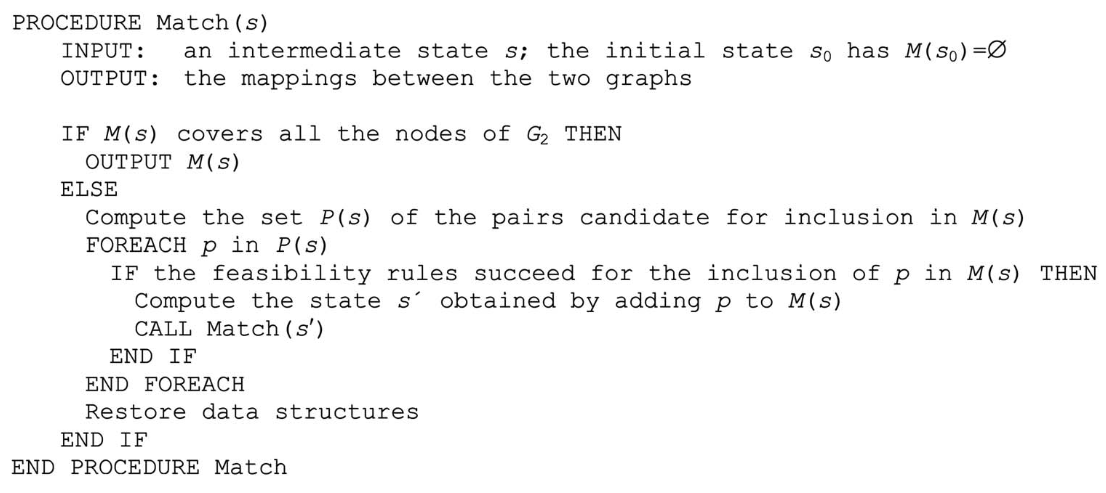
\includegraphics[scale=0.7]{images/vf2_rules.png}
    \caption{Description of the VF2 Algorithm.}
    % use \ref{fig:vf2algo} to refer to this figure in text
    % not that you do anyway
    \label{fig:vf2algo}
  \end{figure}

  For each mapping $(m,n)$, VF2 applies five feasibility rules to the current state and the pair to be added. These rules are denoted as: $R_{pred}, R_{succ}, R_{in}, R_{out},$ and $R_{new}$. Only if all feasibility rules are satisfied is $(n,m)$ added to the set of mappings $M(s)$. The general form of the feasibility function is defined as:

  \[ F_{syn}(s,n,m) = R_{pred} \land R_{succ} \land R_{in} \land R_{out} \land R_{new} \]

  $R_{pred}$ and $R_{succ}$ represent the predecessors and successors respectively of a given node \texttt{n}  in a graph. The other three feasibilty rules are meant to prune the tree. $R_{in}$ and $R_{out}$ are both 1-step ahead look ahead while $R_{new}$ is a 2-step look ahead. ``Look ahead'' refers to the \texttt{k-look-ahead} rules defined in the paper. They are used to reduce the number of states generated, by checking in advance if a consistent state \texttt{s} has no consistent successors after \texttt{k} steps.

  The feasibility rules are defined as follows:

  \begin{figure}[H]
    \centering
    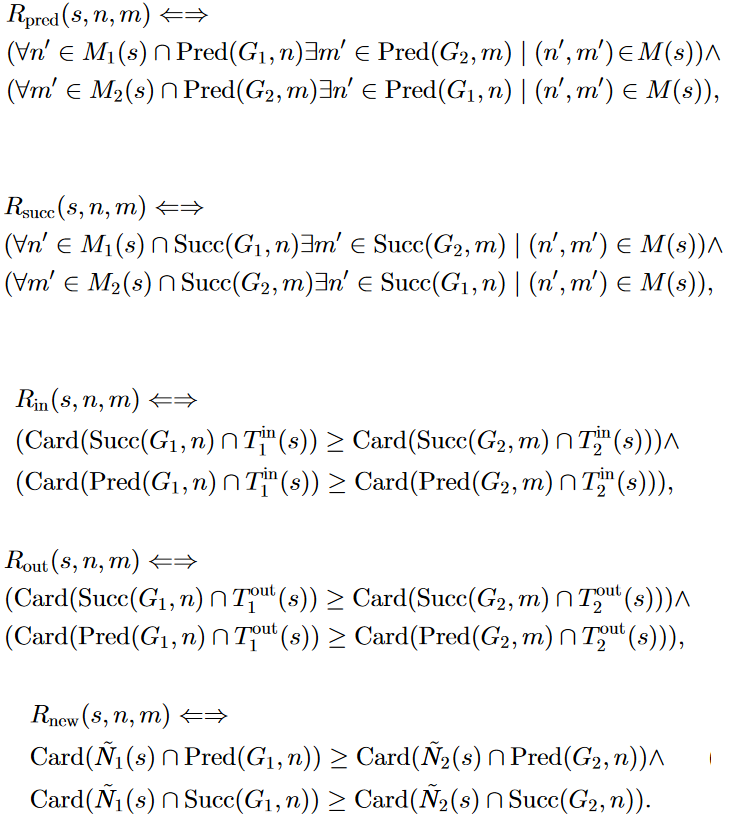
\includegraphics{images/vf2_algo.png}
    \caption{Description of the feasibility rules.}
    \label{fig:vf2feas}
  \end{figure}

  When working with graphs with more than 200 vertices, VF2 typically performs better than Ullmann's algorithm. The time complexity of VF2 is O$(n^2)$ at best, and O$(n!n)$ at worst. Ullmann's algorithm ranges from O$(n^3)$ to O$(n!n^2)$.\cite{cordella}

  \subsection{RI Algorithm}

  For this algorithm, we need to generate all possible maps between two graphs, then check if any of those maps is a subgraph isomorphism.

  The maps can be represented using a \textit{search space tree}, which has a dummy root. Each node represents a possible match between a vertex in graph $G$ (which is referred to as the pattern graph) in the target graph $G'$.

  Unlike other algorithms, RI orders the vertices of the pattern graph in a way that maximizes the chance that a partial path will be removed. The idea is to introduce edge constraints as early as possible, and are modeled only on the pattern graph.

  RI is also modeled for directed graphs, which allows for more pruning since $(u,v)$ does not imply $(v, u)$ (where $u, v$ are vertices).

  The majority of the work is performed in a greedy algorithm called \texttt{GreatestConstraintFirst}, which is used to find a good sequence of vertices based on the number of neighbors a vertex has.

  Using the results of \texttt{GreatestConstraintFirst}, the following isomorphism rules remove unfeasible paths:

  \begin{figure}[H]
    \centering
    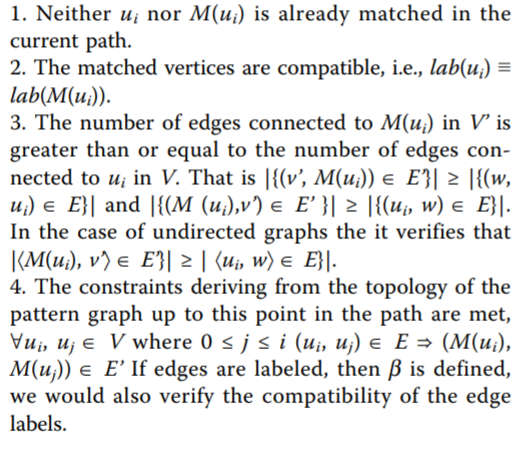
\includegraphics{images/ri_rules.png}
    \caption{RI Feasibility Rules}
    \label{ri_feas}
  \end{figure}


  The algorithm does not have a dedicated pruning function, which is another factor for the increase in performance when compared against other algorithms (such as VF2); instead, pruning is done through the matching process.\cite{bonnici}

\section{Implementation of the Algorithm}

The full source code for all versions can be found in the appendix.

  \subsection{Python Implementation}
  The Python code is based largely on an implementation of the Ullmann algorithm provided by an answer on the website \textit{StackOverflow}.\cite{pyiso} It would not run in its original form, so a few adjustments were needed.

  % restart counting figure numbers
  \setcounter{figure}{0}
  \begin{figure}[H]
    \centering
    \begin{lstlisting}[language=Python]
    def find_isomorphism(graph, subgraph):

        assignments = []
        possible_assignments = [[True]*graph.n_vertices() \
                      for i in range(subgraph.n_vertices())]
        if search(graph, subgraph, assignments, possible_assignments):
            return True
        return matches
    \end{lstlisting}
    \caption{Function used to determine whether an isomorphism exists.}
    \label{ls:findisopy}
  \end{figure}

  The main function is \texttt{find\_isomorphism}, which is depicted above. It calls the function \texttt{search}, which performs the actual work of finding an isomorphism.

  The \texttt{search} function runs  the \texttt{update\_possible\_assignments} function. This particular function has been the subject of refining over the course of the project. At the time of the python implementation, it was the most significant bottleneck.

  This was mostly due to the usage of the \texttt{has\_edge} method of the graph class, shown below.

  \begin{figure}[H]
    \centering
    \begin{lstlisting}[language=Python]
    def has_edge(self, vert1, vert2):
         """ Checks if edge connecting vert1 and vert2 is in the graph
         """
         #if adjacent, there's an edge
         return ({vert1, vert2} in self.adjacencies)

    \end{lstlisting}
    \caption{Code for the \texttt{has\_edge} method of our graph class.}
    \label{ls:hasedgepy}
  \end{figure}

  This method calls the built-in \texttt{in} function of Python lists, which has a runtime complexity of O(n).\cite{bigopy} Thus, the \texttt{has\_edge} method of the Python implementation is O(n).

  \subsection{Initial C++ Implementation}

  The initial C++ implementation was based entirely on the Python implementation. Indeed, it represented our best attempt to ``translate'' the Python code to C++. As one might imagine, it was riddled with compilation errors. That said, we did manage to get it to run, and analysis indicated it performed little better than the Python equivalent. We suspected this was because it retained the same issue that the Python implementation had: calling \texttt{has\_edge}, an O(n) method, countless times. This motivated a significant improvement.

  \subsection{Improved C++ Implementation}

  The improved C++ implementation represents a significant milestone in our project, as it not only improved upon the clarity of the isomorphism algorithm, but also resulted in a much cleaner graph class, with edges implemented as an adjacency matrix. This makes the \texttt{has\_edge} function O(1), as it consists of simply looking up whether the given vertices share an edge by checking the matrix. This makes its repeated use in \texttt{refine\_possible\_assignments} much more acceptable, a fact which is reflected in the performance.

  We also have stored vertices in such a way that each vertex is also stored along with its degree, allowing quick and easy lookup of a vertex's degree.

  The improved C++ implementation follows a bit of a loose interpretation of Ullmann's description of the algorithm. A version which used the \texttt{goto} command with labels was considered, to more closely match said description, but was scrapped in favor of a more conventional approach

  \subsection{Options for Parallelization}

    \subsubsection{GPGPU}
    When GPUs (graphics processing units) began including programmable shaders and support for floating point arithmetic, they became capable of doing calculations on matrices or vectors. While early GPGPU programming (General Purpose computing on Graphics Processing Units) required formulating problems as a series of graphical operations, there are now several APIs available which allow programmers to program directly on GPUs as they would normally.

    One of these APIs is CUDA, which is a proprietary parallel computing platform created by Nvidia. Source code written in CUDA uses C++ syntax, and only Nvidia GPUs are enabled for CUDA. It has the potential to use more than the available cores from a standard CPU, and is only limited by the number of cores that the GPU contains. This ranges from 8 to 5760 (at the time of writing, the Titan Z has 5760 CUDA cores). The main difference between using CUDA and OpenMP is that CUDA has access to many more threads. OpenMP relies on using the cores of a CPU to do parallel work; as a result, work is sped up by approximately a factor of $2^8$, depending on how many cores a computer has.

    A similar API is OpenCL (Open Computing Language), a framework that allows programs to execute accross multiple types of processing hardware. Similar to CUDA, source code is written using C-like syntax. Unlike CUDA, it does not require specialized hardware; OpenCL is an open standard, which can be used across AMD, Nvidia, and Intel GPUs, as well as other processors. However, it is notoriously difficult to both set up for use, and to use.

    \subsubsection{MPI}
    MPI stands for Message Passing Interface. This utilizes multiple machines in order to parallelize the work. Unfortunately there is a large difference between parallelization using multithreading and MPI. With MPI, the function runs once on each machine, rather than running in multiple threads on a single machine. This means that in order to increase effectiveness, the workload must be balanced among the machines, otherwise some machines might do much more work than other machines, reducing the effective time saved. While load-balancing is a concern for all forms of parallelization, it is especially important when using MPI, since a program running in parallel using MPI is only as fast as the slowest machine, and there is a large amount of overhead in having to send each machine's results across a local network to other machines for further processing. Thus, one cannot simply use MPI to parallelize a program and expect it to perform faster by some predetermined factor. In the case of graph and subgraph isomorphism, we would have to split the work based on which sections of the graph take longer to find mappings for.

    Theoretically, it is possible to combine MPI with OpenMP in order to further increase the efficiency. However, our team did not have a network of machines in order to use MPI. If we did, the time it would take to find an isomorphism would decrease by at most a factor based on the number of processors used, multiplied by the number of cores in each processor capable of using OpenMP.

    \subsubsection{SIMD}
    SIMD (single instruction, multiple data) uses a series of data types, which can be utilized on CPUs that support them. These data types allow for data level parallelism, similar to OpenMP. Examples of SIMD instructions that utilize these data types are AVX, SSE, and ARM-NEON vector instructions. These instructions allow for operations to be done on these data types on multiple sections at once. For example, when iterating through a loop, we can load four values of an array and add them all at once in a single operation, rather than loading them one at a time into a separate variable to be added. This would allow the program to only iterate one fourth as many times to complete the computation. Other operations can either be between two vectors or between values within the vectors. However, taking advantage of SIMD programming would have required us to drastically alter the data structures we currently have in place to incorporate SIMD datatypes.

  \subsection{Optimizations through OpenMP}
  Ultimately, we decided to settle on using OpenMP. OpenMP utilizes the multiple cores of a computer's processor in order implement multithreading to run related tasks in parallel. We intend to use it where the bottlenecks in our algorithm are to improve the algorithm's performance. The default number of cores for many computers is four. We intend to place the parallelisms where there tend to be a large number iterations, specifically in loops. This means that, theoretically, the program should run four times faster than without multithreading, using our earlier assumption of four processor cores allotted to the algorithm. It is more likely that it will be approximately 3 to 3.5 times faster, since we may not be able to completely parallelize the bottlenecks as intended. Additionally, using OpenMP, as is the case with any parallelization method, comes with a certain amount of overhead in separating the work to be done. There is also the issue of load balancing: making sure that each thread is performing approximately the same amount of computation so that no thread is idling.

  The most important place to place the OpenMP is in the \texttt{refine\_possible\_assignments} function. This function is where the majority of the algorithm's computation takes place, as it has several layers of nested loops, each iterating through vectors which may be very large, depending on the sizes of the graphs being examined. Ideally, we want to balance the loads such that each processor core does an equal amount of work, so as to maximize the amount of parallelization done. However, while we may simply parallelize every iterative process, that might not be efficient enough. Ideally, we would further parallelize in nodes of the search tree which have many possible assignments.

  \subsection{Sample Run}

  For visualization purposes, we have provided a sample run of the algorithm. For simplicity, only the C++ implementation is seen here. The graphs used are very simple, as this is only for demonstration. The following is the list of edges defining the search graph:

  % restart counting figure numbers
  \setcounter{figure}{0}
  \begin{figure}[H]
    \centering
    \lstinputlisting{../../src/toy1.edges}
    \caption{Search graph used for walkthrough.}
    \label{ls:toysearch}
  \end{figure}

  The following is the subgraph we will be searching for an instance of in that graph:

  \begin{figure}[H]
    \centering
    \lstinputlisting{../../src/toy1sub.edges}
    \caption{Subgraph being searched for in search graph.}
    \label{ls:toysub}
  \end{figure}

  We can place these into text files, named \texttt{example.edges} and \texttt{sub.edges} for figures \ref{ls:toysearch} and \ref{ls:toysub}, respectively. With these filenames, and assuming the program executable is a file in the same directory named \texttt{main}, we may run the program from the terminal using the command \texttt{./main example.edges sub.edges}. That is, we pass the text file specifying the search graph in as the first argument, and the corresponding file for the subgraph as the second argument.

  The program may also be run in interactive mode by passing in the argument \texttt{-i} or \texttt{--interactive}, in which case the user is prompted to enter the list of edges for each graph manually in the terminal. This allows for manual entering of the graphs in case files are not available for whatever reason, or for testing simple cases that are not worth creating files for. A full list of arguments along with usage information can be viewed by running the program with the \texttt{-h} or \texttt{--help} arguments. 

  After the two files are parsed and the corresponding graph objects are created, the program runs \texttt{find\_isomorphism} with the subgraph and search graph as arguments, which returns a vector of assignments from the subgraph vertices to the search graph vertices, or an empty vector if no isomorphism exists.

  Note that, at this point, the search graph consists of a graph with vertices $(1, 2, 3)$, and the subgraph consists of vertices $(10, 20)$.

  In \texttt{find\_isomorphism}, we first set up the matrix of possible assignments M by running \texttt{vector < vector<bool> > possible\_assignments = create\_possible\_assignments(sub, graph);}. This creates the matrix by initializing a vector of size $p_{\alpha}$, populated with $p_{\alpha}$ vectors of size $p_{\beta}$. Each of the values in these vectors is initialized to false. This is all done in one line using one of the constructors provided by the C++ vector class. We then use a nested for loop to iterate through each position of the matrix, setting the position to true if the vertex corresponding to the current column in the search graph has a degree greater than or equal to the degree of the vertex corresponding to the current row in the subgraph. Our graph class stores vertices as pairs of integers. The first integer is the unique value associated with the vertex, and the second integer is the degree of the vertex. The degree is incremented every time a pair which contains the vertex is added to the graph. This way, looking up degree of a vertex is trivial. \texttt{create\_possible\_assignments} returns the matrix created.

  The next step is to initialize the various variables used to keep track of our place in the computation. The first of these is \texttt{assignments\_tree}, which is a vector of max size $p_{\alpha}$ that will contain the matrix of possible assignments at each depth. This is so that we have a way to access the previous matrices in the event that we need to backtrack. The next variable we need is \texttt{cols\_used}, which keeps track of which columns (corresponding to search graph vertices) have already been assigned to a row (corresponding to subgraph vertices). \texttt{cols\_used[i] == true} if column \texttt{i} has been assigned. Each search graph vertex can only be assigned to a single subgraph vertex, so it is important to keep track of which columns have already been assigned. The next variable we will need is \texttt{col\_depth}. \texttt{col\_depth[i-1] == k} if column \texttt{k} was assigned to a row at depth \texttt{i}. The need for this will become clear later on in the example, but in simple terms it is used to keep track of what the last column we tried to assign to a row was, so that we do not continually attempt to assign the same column to the same row after determining doing so does not lead to an isomorphism. The final variable is self-explanatory: \texttt{depth}. This initialized to 1, and keeps track of our depth in the search tree, if we represent the sets of all possible assignments as a search tree, with isomorphisms at depth $p_{\alpha}$ if they exist.

  Finally, we pass all of these variables along with the subgraph and search graph to the \texttt{search} function, which returns true if an isomorphism is found, and false otherwise. At this point, matrix M consists of:
  
  \[ \begin{pmatrix}
      1 & 1 & 1 \\
      1 & 1 & 1
  \end{pmatrix} \]

  Since every vertex in the search graph has degree $\geq 1$, every vertex is a possible assignment for every vertex in the subgraph.

  The first thing we do in \texttt{search} is refine matrix M. This is done first, so that, if the refinement fails, we will know right away, and avoid having to do any unnecessary work. We place the call to the function as the conditional to an if statement. If it returns false, we go into the body of the if statement, which contains only the statement \texttt{return false;}, indicating that no isomorphism was found.

  In the refinement procedure, to which we have passed the matrix of possible assignments and the two graphs, the first noteworthy variable is the boolean \texttt{changes\_made}, which is keeps track of whether or not we have made any changes to the possible assignments matrix. Since eliminating a possible assignment may make other possible assignments invalid, we must run the refinement procedure on the matrix repeatedly to eliminate these newly-invalid assignments. This may occur several times, so we have a variable to keep track of when we can stop. Thus, the entire procedure is wrapped in a while loop, with \texttt{changes\_made} being the conditional. In the while loop, we first set \texttt{changes\_made} to false, and we will set it to true if we mark any possible assignment as invalid.

  For convenience, here is the current state of possible assignments once again:

  \[ \begin{pmatrix}
      1 & 1 & 1 \\
      1 & 1 & 1
  \end{pmatrix} \]

  We first iterate through each of the rows using a simple for loop. That is, we check each subgraph vertex's possible assignments for validity. The next noteworthy variable is the boolean \texttt{no\_one}, which is initially true. This variable, which may be confusingly-named, keeps track of whether or not the current row contains no possible assignments. If this is true, we stop the procedure entirely and return false, since it is no longer possible for an isomorphism between the two graphs to exist. Thus, continuing to prune possible assignments is a pointless effort if we have already found there are no possible assignments for any given row. We then iterate through each column of the current row. If the column is a possible assignment of the current row, we first set \texttt{no\_one} to false since the current row has at least one possible assignment.

  The next step is to look through all neighbors of the subgraph vertex corresponding to the current row. Since our subgraph consists only of two vertices, the set of neighbors in this case contains a single member. We use an iterator and a for loop to iterate through the set of neighbors of the current row's vertex. This set is provided by the graph class's \texttt{neighbors} method, which returns the set of neighbors of the vertex passed to it. For each of the row's neighbors $n_i$, we iterate through its possible assignments. We use the boolean value \texttt{has\_corresponding\_neighbor} to track whether or not the row's neighbor has a possible assignment which is a neighbor of the vertex corresponding to the current column. At each possible assignment of $n_i$, we check whether or not the corresponding vertex in the search graph has an edge connecting it to the current column, which is in turn a possible assignment of the current row. If such an edge exists, then we mark \texttt{has\_corresponding\_neighbor} true, and check the next neighbor.

  If the current row has no neighbors which are neighbors of the current column, then \texttt{has\_corresponding\_neighbor} is never set to true, so we set the current column and row of possible assignments to false, and set \texttt{changes\_made} to true.

  Unfortunately for us, there are no invalid assignments in the possible assignments matrix, so the refinement procedure returns true without changing the matrix. Here it is again, for convenience:

  \[ \begin{pmatrix}
      1 & 1 & 1 \\
      1 & 1 & 1
  \end{pmatrix} \]

  We thus continue in \texttt{search}. Since the refinement procedure returned true, the if block is not executed, and we instead go onto a do..while loop. This was structured as a do..while, since we may need to iterate several times, but we would still like to execute the block at least once. We would later find that this was irrelevant, since the condition we used was \texttt{while(true)}, an infinite loop. Our reasoning for this should soon become apparent. 
  
  The next step is to initialize several variables for use in loops; nothing worth calling attention to. We enter a for loop to iterate through columns of the current row (the current row being given by \texttt{depth-1}), initializing the iterating variable \texttt{col} to \texttt{col\_depth[depth-1]}. We stop iterating once \texttt{col < numcols}, the latter of which should be self-explanatory. Once we find a possible assignment from the current row to a column, we check if that column has already been used by checking \texttt{cols\_used[col]}. If so, we continue iterating to find another column. If not, we break out of the loop.

  The first thing we do after breaking from the loop is to check whether \texttt{col} is equal to \texttt{numcols}. If so, this means we couldn't find a valid column to assign the current row to, so we must backtrack to the previous row to attempt to assign it to a different column. We do this by decrementing \texttt{depth} by 1, setting the possible assignments matrix to the one stored at \texttt{assignments\_tree[depth-1]} (note that this the new value of depth), and returning false. If we are at depth 1, then there is no previous row to reassign, and we simply return false. In our particular example, since we haven't used any columns and every entry in the possible assignments matrix is true, \texttt{col} is 0 after exiting the for loop, and \texttt{numcols} is obviously 3. Thus, we do not enter the block of the if statement.

  Since we have found a valid column to assign to the current row, we set all other columns in the current row of possible assignments to false, along with all other rows in the current column. For us, that means all other columns in row 0 and all other rows in column 0. This yields the following matrix of possible assignments:

  \[ \begin{pmatrix}
      1 & 0 & 0 \\
      0 & 1 & 1
  \end{pmatrix} \]

  With one row assigned, we must recursively search for an isomorphism under this new matrix of possible assignments. We do this by calling \texttt{search} again, but with modified arguments. Namely, we append the current matrix of possible assignments to the assignments tree variable in case we need to backtrack later, we set \texttt{cols\_used[col]} to true to indicate that the column \texttt{col} has been used, set \texttt{col\_depth[depth-1]} to \texttt{col}, and increment \texttt{depth}. At this point, we check if \texttt{depth} is equal to $p_{\alpha}$ and, if so, return true, since that means every row has been assigned to a column. In our case, since there are only two rows, and \texttt{depth} is equal to 2, we return true. Note that this still leaves extra possible assignments in the bottom row of the possible assignments matrix. We simply ignore these and assign the bottom row to the first possible assignment in it. 
  
  If we'd had more rows, then the if block would not have executed, and we would have instead entered a different if statement which runs \texttt{search} recursively using the modified variables as arguments. If this search returns true, we have found an isomorphism under the modified possible assignments matrix, and we return true to report this finding. If it does not return true, then we set \texttt{cols\_used[col]} back to false and return to the top of the while loop to try a new column. Since we had already set \texttt{col\_depth[depth-1]} to \texttt{col}, we do not have to worry about the algorithm attempting to assign this row to the same column with the same result. It will continue attempting to reassign \texttt{col} starting from the next column.

  The final state of our possible assignments matrix after returning is thus:

  \[ \begin{pmatrix}
      1 & 0 & 0 \\
      0 & 1 & 1
  \end{pmatrix} \]

  Since we returned true from \texttt{search}, we extract the set of possible assignments at the lowest depth in the tree that we ended on. That is, we set the assignments list to \texttt{assignments\_tree[depth-2]}. We subtract 2 from \texttt{depth}, since we incremented \texttt{depth} by 1 before returning from \texttt{search}, so the list of assignments we want is actually at index \texttt{depth-2}. After assigning this to a variable we call \texttt{assignments}, we create a new vector called \texttt{isomorphism}, which contains the actual mappings which will be returned. To populate \texttt{isomorphism}, we iterate through the \texttt{assignments} matrix. Whenever we come upon an assignment, we push the current column number onto the \texttt{isomorphism} vector. In this way, \texttt{isomorphism[i]} is the vertex in the search graph assigned to vertex \texttt{i} in the subgraph. After pushing the column number, we break to go to the next row. Since each row can only have one possible assignment, there is no need to continue iterating through columns after we've found the assignment for a particular row. This also means that the bottom row, which may have multiple assignments, will have only the first of its assignments added to the vector, with the rest ignored.

  Finally, after getting the assignments into a vector, we return the \texttt{isomorphism} vector. It is worth noting that, had we returned false from \texttt{search}, the if block would not have executed, and we would have instead returned an empty vector to indicate no isomorphism exists.

  Back in the main function, we first check if the returned vector is empty. If so, no isomorphism was found, and we take action accordingly. In this case, we simply print a message indicating that no isomorphism was found. However, an isomorphism \textit{was} found, so the return vector is a vector of assignments. We thus print a message indicating that an isomorphism was found, and print out which vertices in the subgraph map to which vertices in the search graph. We can retrieve the original values of the vertices given their indices by using the graph class method \texttt{get\_value}, which takes the index of a vertex and returns the value of the vertex at that index in the vector of vertices in the graph. For example, for our subgraph, the vertex 10 has index 0, so \texttt{get\_value(0)} will return 10. This way, we do not need to actually store the vector values along with the isomorphism vector; we can simply retrieve them afterwards. In our case, we have found that subgraph vertex 10 can be mapped to search graph vertex 1, and subgraph vertex 20 can be mapped to search graph vertex 2. 
  
  Since the graphs are quite small, it is trivial to draw them and verify that this result is correct. Indeed, it is one of a number possible correct results, but we only return the first one found. Future improvements to the project may include listing all possible isomorphisms, or at the very least counting them.

\section{Performance}

For all of our measurements, we used the worst-case input: the Facebook graph mentioned previously as the search graph, and that same graph (or, equivalently, any isomorphic graph of the same size) as the subgraph. This would take the longest of the graphs available to us, since it requires the algorithm to assign the greatest number of vertices (all of them) before returning, and, since the graphs are indeed isomorphic, there is no chance of \texttt{refine\_possible\_assignments} returning false, which would allow us to skip a large amount of work.

  \subsection{Python Implementation}
  The Python implementation was very inefficient, but it was necessary for us to understand what we had to do for a C++ implementation. It took between 13 and 16 seconds to determine if an isomorphism existed.

  We used the Python \texttt{cProfile} library to measure the performance of our Python implementation. The documentation is available at \url{https://docs.python.org/3.5/library/profile.html}. A typical run of the \texttt{find\_isomorphism} function timed by \texttt{cProfile} produces the following output:

  \begin{figure}[H]
    \centering
    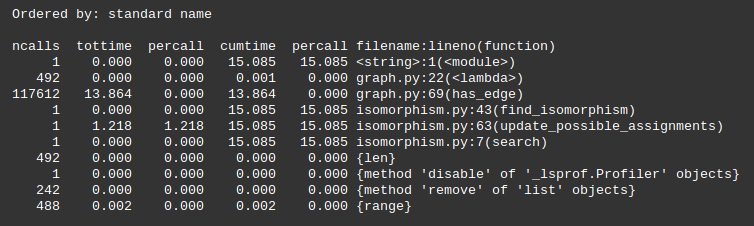
\includegraphics[scale=0.6]{images/perf}
    \caption{Sample run of the Python implementation of subgraph isomorphism.}
  \end{figure}

  We see that, as previously explained, the overwhelming majority of the time was spent in \texttt{update\_possible\_assignments}, specifically running \texttt{has\_edge}, which in turn calls the \texttt{in} function. The \texttt{has\_edge} method is called over 117 thousand times. This is the key bottleneck in the algorithm, and any amount of improvement in that particular aspect is likely to lead to huge performance improvements, given how many times \texttt{has\_edge} is called.

  \subsection{C++ Implementation}

    \subsubsection{Performance Tradeoffs}
    While our graph class is remarkably efficient at determining whether a particular edge exists between two vertices, as well as determining the degree of a particular vertex, this efficiency is not without drawbacks. Most notably, storing a binary matrix of edges brings the space complexity of our graph class up to O$(n^2)$. Memory is very cheap in this day and age, so sacrificing it for performance (which, as we will see, is much better) was acceptable for our purposes. This is, however, something to keep in mind for future implementations.

    Additionally, updating this matrix whenever an edge or vertex is added to the graph adds considerable overhead in itself, making \texttt{add\_edge} and \texttt{add\_vertex} more expensive methods to run.

    \subsubsection{Results}
    The source code used to test the performance of the C++ implementations can be found in the appendix. We used Linux's \texttt{perf\_event\_open} system call, which allows for high-precision performance monitoring. The only part of the program which is timed is the call to \texttt{find\_isomorphism}.

    The C++ implementation, due to the improvement of \texttt{has\_edge}'s runtime, runs significantly more quickly than the Python implementation; it runs in about 8 seconds, compared to about 16 seconds for the Python implementation. This is about twice as fast, even without any parallelization. However, we found it was generally more precise to measure the number of CPU clock cycles taken for the algorithm to complete, so we measured that instead. The output of the program used to measure this is below:

  \setcounter{figure}{0}
  \begin{figure}[H]
    \centering
    \lstinputlisting{cperf.txt}
    \caption{Performance of non-parallelized version of our algorithm.}
    \label{ls:cperf}
  \end{figure}

  We see that the C++ version took 26,142,295,153 cycles to complete on the system used to test. This is equivalent to about eight seconds, as mentioned previously. The exact number of cycles will vary slightly from trial to trial, but repeated trials have made us confident that this is a representative sample.

  \subsection{OpenMP Optimization}
  The OpenMP code performs very well compared to the non-parallelized version. The system we tested it on has a four-core CPU, allowing for up to four threads to run in parallel, leading to a four-fold performance improvement. It is important to note, however, that even in the case of absolute perfect parallelization, it is impossible to achieve exactly four times the performance. Using OpenMP requires the program execution to split up into four threads and combine back into one after each of the four threads have finished the work assigned to them. This necessitates the execution of a few additional instructions beyond the ones relevant to the computation in our algorithm. Thus, even in the best case, we can only hope for performance which is slightly less than four times faster.

  Moreover, we must consider the fact that we are not parallelizing the entire algorithm; only \texttt{refine\_possible\_assignments} is run in parallel, and only part of it, at that. The rest of the algorithm runs serially, like the non-parallelized version. Thus, even without the overhead involved with using OpenMP, we cannot ever expect the entire algorithm to run four times faster, when only part of it runs (theoretically) four times as fast. 

  With all that said, we came surprisingly close to four times faster, all things considered. The output of the program used to measure the performance of the OpenMP code is below:

  \setcounter{figure}{0}
  \begin{figure}[H]
    \centering
    \lstinputlisting{ompperf.txt}
    \caption{Performance of OpenMP version of our algorithm.}
    \label{ls:ompperf}
  \end{figure}

  Here we see instead that the algorithm now takes only 7,125,381,701 cycles to complete. Once again, this number will vary slightly for each run, but this particular number was about average. Using the number from figure \ref{ls:cperf}, we can compute how much faster this particular run of the parallelized algorithm is than that particular run of the non-parallelized algorithm by dividing the latter by the former. This comes out to:

  \[ \frac{26142295153 \mathrm{ cycles}}{7125381701 \textrm{ cycles}} \approx 3.669 \]

  At 3.669 times faster, the parallel version of the algorithm runs much closer to four times faster than we had anticipated, given the factors discussed earlier. This greatly supports our hypothesis that parallelizing just the refinement procedure leads to a much more efficient implementation, since that function is by far the most computationally expensive portion of the algorithm, and is called many, many times.

\section{Conclusion}
  Using parallelization techniques in order to increase efficiency of the NP-complete problem of subgraph isomorphism proved to be a success. In our C++ implementation of Ullman's algorithm with OpenMP, graph isomorphism took two to three seconds to compute; this is down from the average of eight seconds from the C++ implementation without parallelization, using what was easily our worst-case scenario. Additionally, solving smaller instances of the subgraph isomorphism problem take less than a second. In either case, using C++ and adding OpenMP optimizations resulted in a much faster implementation than our Python implementation, which took between 14 and 16 seconds to run. 
  
  When it comes to innovation, everyone wants their next thing to be more efficient, both time-wise and space-wise. This project has shown that even the smallest amount of parallelization can make a large difference for very complex problems. If we had combined various parallelization techniques, such as utilizing SIMD instructions alongside the multithreading technique we used, we might have gotten an implementation even faster than what we had. Parallelization is seeing growing usage to address the problems of an increasingly demanding world.

\section{Appendix}
  \subsection{Python Code}
    \subsubsection{Graph Class}
      \lstinputlisting[language=Python,caption={Python graph class.}]{../../src/pythonvers/graph.py}
    \subsubsection{Subgraph Isomorphism Algorithm}
      \lstinputlisting[language=Python,caption={Python algorithm to find isomorphism.}]{../../src/pythonvers/isomorphism.py}
    \subsubsection{Main}
      \lstinputlisting[language=Python,caption={Python main function to process arguments and run the ismorphism algorithm.}]{../../src/pythonvers/main.py}

  \subsection{C++ Code}
    \subsubsection{Graph Class}
      \lstinputlisting[language=C++,caption={C++ graph class.}]{../../src/cvers/graph.cpp}
    \subsubsection{Subgraph Isomorphism Algorithm}
      \lstinputlisting[language=C++,caption={C++ algorithm to find isomorphism.}]{../../src/cvers/isomorphism.cpp}
    \subsubsection{Main}
      \lstinputlisting[language=C++,caption={C++ main function to process arguments and run the ismorphism algorithm.}]{../../src/cvers/main.cpp}

  \subsection{OpenMP Code}
    \textbf{Note:} Since the OpenMP version of our algorithm uses the same graph class and \texttt{main.cpp}, we have omitted them from this section.

    \subsubsection{Subgraph Isomorphism Algorithm}
      \lstinputlisting[language=C++,caption={C++ algorithm to find isomorphism, with parallelisms through OpenMP.}]{../../src/openmp/isomorphism.cpp}

  \subsection{Code Used to Check Performance of C++ code}
    % if you've got a better caption be my guest
    \lstinputlisting[language=C++,caption={Code used to check performance of C++ code}]{../../src/cvers/perf.cpp}

  \printbibliography[heading=bibintoc,
                     title={References}]

\end{document}
